\documentclass[10pt]{report}
\setcounter{tocdepth}{4}
\setcounter{secnumdepth}{4}

% Insert ToC-writing after starting a titlepage
\usepackage{etoolbox}
\patchcmd{\abstract}{\titlepage}{\titlepage \addcontentsline{toc}{chapter}{Abstract}}{}{}

% to insert a title at the beginning of each page
% http://ctan.mirror.garr.it/mirrors/CTAN/info/italian/fancyhdr/itfancyhdr.pdf
\usepackage{fancyhdr}
\pagestyle{fancy}
\lhead{}
\rhead{}
\chead{Micro Simplified Hayekian Market}


\usepackage{geometry}            % See geometry.pdf to learn the layout options. There are lots.
\geometry{a4paper}                   % ... or a4paper or a5paper or ... letterpaper
%\geometry{landscape}                % Activate for for rotated page geometry
%\usepackage[parfill]{parskip}    % Activate to begin paragraphs with an empty line rather than an indent
\usepackage{graphicx}
\usepackage{amssymb}
\usepackage{epstopdf}
\usepackage[hyphens]{url}         %[hyphens] to break long urls
\usepackage{t1enc} %per uso di caratteri come << >>
%\DeclareGraphicsRule{.tif}{png}{.png}{`convert #1 `dirname #1`/`basename #1 .tif`.png}

\usepackage{verbatim} %to use \begin{comment} \end{comment}
\usepackage{float} % to use H as rigid placement of a figure after the text, allowing empty spaces

\usepackage{fancyvrb}  % http://texdoc.net/texmf-dist/doc/latex/fancyvrb/fancyvrb.pdf

\usepackage{enumitem} % to avoid bold in description item and to maintain bullets

\usepackage[toc,page]{appendix}

\usepackage{keystroke} % to use \Return

\newcommand{\repeatfootnote}[1]{\textsuperscript{\ref{#1}}} %to repeat a reference


% to have clickable links and references
\usepackage[dvipsnames]{xcolor} % colors at https://en.wikibooks.org/wiki/LaTeX/Colors
\usepackage{xcolor}   %Maybe necessary if you want to color links (better use xcolor than color, more at http://repositorios.cpai.unb.br/ctan/macros/latex/contrib/xcolor/xcolor.pdf)
\usepackage{hyperref}
\hypersetup{
    colorlinks=true, %set true if you want colored links
    linktoc=all,     %set to all if you want both sections and subsections linked
    linkcolor=Brown,  %choose some color if you want links to stan
    urlcolor=cyan,
    citecolor=purple}
    
\usepackage{chngcntr}                      % to avoid restart note numbers 
\counterwithout{footnote}{chapter}    % changing chapter

\usepackage{makeidx}   % creating index (in Italian Indice analitico)

\usepackage{empheq}

\usepackage{tablefootnote} % to use \footnote as \tablefootnote

\newcommand{\ts}{\textsuperscript} %to write briefly th etc. as a superscript

\usepackage{color}
\usepackage{listings}



\makeindex



\title{Micro Simplified Hayekian Market}
%\subtitle{a}
\author{Matteo Morini\footnote{University of Torino, Italia} and Pietro Terna\footnote{University of Torino, Italia}}

%\date{} %attivare vuoto per eliminare la data oppure attivarne una dichiarata

%\usepackage[square]{natbib}
\usepackage[round]{natbib}

\setlength\fboxsep{0pt}

\renewcommand{\thesection}{\arabic{section}} % to avoid leading zeros in numbering the sections, having eliminate
                                                                           % the Chapter 1 supertitle (see below: to eliminate the Chapter 1 
                                                                           % supertitle)


\begin{document}
\maketitle
\thispagestyle{fancy}



%%%%%%%%%%%%%%%%%%%%%%%%%%%%%%%%%%%%%%%%%%%%
%%%%%%%%%%%%%%%%%%%%%%%%%%%%%%%%%%%%%%%%%%%%
\begin{abstract}
\thispagestyle{fancy}

We propose a simplified version of the Hayek's decentralized market hypothesis, considering elementary processes of price adaptation in exchanges.

Sections \ref{The technical setup} and \ref{The structure of the model} report the technical setup and the structure of the model. In Section \ref{The hayekian version} we introduce an elementary agent-based model of a market, with emergent (quite interesting)  price dynamics.

A counter example is also introduced in Section \ref{The unstructured version}, showing that---with tiny modification---we generate implausible price dynamics.

In Appendix \ref{Two triple cases of not balancing numbers of buyers and sellers} we report some technical analyses of the cases with unmatching numbers of buyers and sellers. These analyses are strongly related the the \href{https://terna.github.io/oligopoly/}{Oligopoly}\footnote{Clic to go to \url{https://terna.github.io/oligopoly/}} simulation project.

Appendix \ref{Activating idle agents} will be dedicate \ldots
\end{abstract}
%%%%%%%%%%%%%%%%%%%%%%%%%%%%%%%%%%%%%%%%%%%%
%%%%%%%%%%%%%%%%%%%%%%%%%%%%%%%%%%%%%%%%%%%%


\setcounter{page}{2}
\tableofcontents
\thispagestyle{fancy}


\listoffigures
\thispagestyle{fancy}
\setcounter{page}{2}




%%%%%%%%%%%%%%%%%%%%%%%%%%%%%%%%%%%%%%%%%%%%
%%%%%%%%%%%%%%%%%%%%%%%%%%%%%%%%%%%%%%%%%%%%
\chapter*{Introduction to a Micro Simplified Hayekian Market}
%The * above is to eliminate the Chapter 1 supertitle
\label{micro Hayekian Market}\index{introduction to a micro simplified Hayekian Market}
\thispagestyle{fancy}
\addcontentsline{toc}{chapter}{\protect\numberline{}Introduction to a micro Hayekian Market}%


The purpose of the note is that of introducing a very simple agent-based model of a market, with emergent (quite interesting)  price dynamics.

 A counter example is also introduced, showing how---with tiny modifications---we generate implausible/impossible price dynamics.

The code uses the IPython\footnote{\url{https://ipython.org}} language (an interactive layer upon Python\footnote{\url{https://www.python.org}} using the Jupyter\footnote{\url{http://jupyter.org}} infrastructure) and can be dowloaded from \url{https://github.com/terna/microHayekianMarket} via the \emph{Clone or download} button; it is also possible to run it directly on line thanks to the \href{https://mybinder.org/v2/gh/terna/microHayekianMarket/master?filepath=microHayekianMarket.ipynb}{MyBinder project}\footnote{Click to go to \url{https://mybinder.org/v2/gh/terna/microHayekianMarket/master?filepath=microHayekianMarket.ipynb}}.

A suggested reading about Hayek is a quite recent paper of \citeauthor{10.1257/jep.31.3.215} (\citeyear{10.1257/jep.31.3.215}).

Quoting from the introduction:
\begin{quotation}
Friedrich A. Hayek (1899-1992) is known for his vision of the market economy as an information processing system characterized by spontaneous order, the emergence of coherence through the independent actions of large numbers of individuals each with limited and local knowledge, coordinated by prices that arise from decentralized processes of competition.
\end{quotation}

A simplified version---proposed here---is that of considering decentralized elementary processes of price adaptation in exchanges, with surprising results.

%%%%%%%%%%%%%%%%%%%%%%%%%%%%%%%%%%%%%%%%%%%%
\section{The technical setup}\label{The technical setup}\index{technical setup}

The IPython (or Python 3.x) code requires the following setup to start:

\begin{lstlisting}[language=Python, caption=Setup of the program, basicstyle=\ttfamily\footnotesize]
%pylab inline
%pylab inline
import statistics as s
import numpy as np
import pylab as plt
from ipywidgets import Output
from IPython.display import clear_output
from IPython.display import display
import time
import math\end{lstlisting}

\verb|%pylab inline| 
is a \emph{magic} command of Jupyter.

%%%%%%%%%%%%%%%%%%%%%%%%%%%%%%%%%%%%%%%%%%%%
\section{The structure of the model and the \emph{warming up} phase}\label{The structure of the model}\index{structure}

Our agents are simply prices, to be interpreted as reservation prices.\footnote{The $max$ price a buyer could pay and the $min$ one a seller could accept.}

We have two price vectors: $pL^b$ with item $pL^b_i$ for the buyers, and $pL^s$ with item $pL^s_j$ for the sellers. The $i^{th}$ or the $j^{th}$ elements of the vectors are prices, but  we can use them also as agents.

Both in the simplified hayekian perspective (Section \ref{The hayekian version}) and in the unstructured one (Section \ref{The unstructured version}) we have to pre-run a \emph{warning up} action. This happens automatically, calling the specific function in the beginning of both the cases.

With the \emph{warming up} phase, we define:

\begin{itemize}
\item $d_0$ - the lower bound of the random uniform numbers, both for the buyers and the sellers, in the warming up phase; 

in the running phase, the lower bound is $0$;
\item $d_1$ - the upper bound of the random uniform numbers for the buyers;
\item $d_2$ - the upper bound of the random uniform numbers for the sellers;
\item $nCycles$ - number of simulation cycles;
\item $nBuyers$  - number of the buyers;
\item $nSellers$ - number of the sellers;
\item $seed$ - the seed of the random numbers;
\item the initial buyer $i$ reservation price, different for each buyer: $p_{b,i}=\frac{1} {1 + u_i}$ with $u_i\sim\mathcal{U}(d_0,d_1)$;
\item the initial seller $j$ reservation price, different for each seller: $p_{s,j}=1 + u_j$ with $u_j\sim\mathcal{U}(d_0,d_2)$;
\item $buyersSellersRatio$ - the ratio $\frac{nBuyers}{nSellers}$;
\item $sellersBuyersRatio$ - the ratio $\frac{nSellers}{nBuyers}$;
\item $usingRatios$ - a logic variable activating limitations to $d_1$ or $d_2$
\item $squeezeRate$ - always $< 1$, as further compression of $d_1$ or $d_2$
\item $usingSqueezeRate$ - a logic variable to further squeeze $d_1$ or $d_2$
\end{itemize}

With  $d_0=0.1$, $d_1=0.2$, $d_2=0.2$, sorting in decreasing order the vector  $pL^b$ and in increasing order the vector  $pL^s$, we obtain in Fig. \ref{output_3_1.png} two not overlapping price sequences that we can interpret as a demand curve (red) and an offer one (blue).

\begin{figure}[H]
\begin{center}
\fbox{\centering 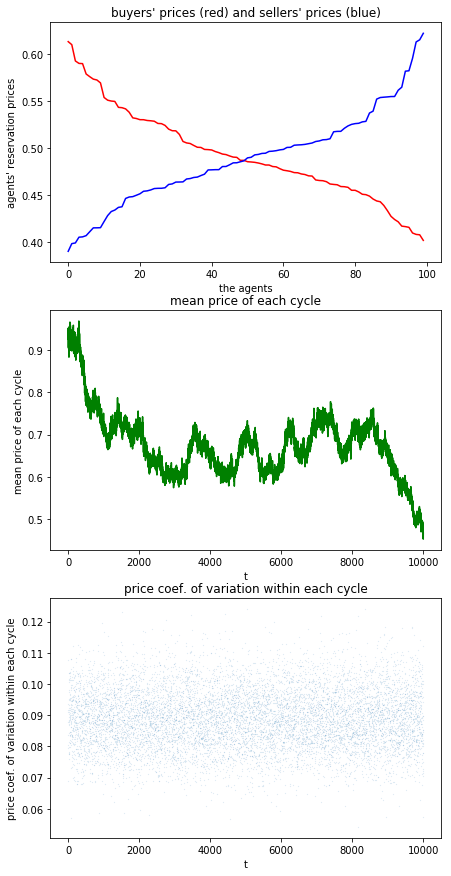
\includegraphics[width=0.6\textwidth]{output_3_1.png}}
\caption{An example of initial not overlapping demand curve (red) and offer curve (blue)}
\label{output_3_1.png}
\end{center}
\end{figure}

To generate new examples related to Section \ref{The hayekian version} and to Section \ref{The unstructured version}, it is necessary to repeat this phase. This happens automatically, calling the specific function in the beginning of both the cases.


The IPython (or Python 3.x) code is:

\begin{lstlisting}[language=Python, caption=Warming up of the model, basicstyle=\ttfamily\footnotesize]
# warming up

# execute before both: 
#                     - the hayekian perspective or
#                     - the unstructured case
def warmingUp():
    global nCycles, nBuyers, nSellers,\
        buyersSellersRatio, sellersBuyersRatio,\
        usingRatios, usingSqueezeRate, squeezeRate,\
        d0, d1, d2, buyerPriceList, sellerPriceList

    nCycles=10000
    nBuyers= 50
    nSellers=100

    buyersSellersRatio=nBuyers/nSellers
    sellersBuyersRatio=nSellers/nBuyers
    usingRatios=True
    squeezeRate=0.3 # always < 1 
    usingSqueezeRate=False

    seed=111
    np.random.seed(seed)

    d0=0.1
    d1=0.2
    d2=0.2


    buyerPriceList=[]
    sellerPriceList=[]

    for i in range(nBuyers):
        buyerPriceList.append(1/(1+np.random.uniform(d0,d1)))
    for j in range(nSellers):
        sellerPriceList.append(1+np.random.uniform(d0,d2))
    
    plt.figure(0)
    plt.plot(sorted(buyerPriceList,reverse=True),"r");
    plt.plot(sorted(sellerPriceList),"b");
    xlabel("the agents");
    ylabel("agents' reservation prices");
\end{lstlisting}

%%%%%%%%%%%%%%%%%%%%%%%%%%%%%%%%%%%%%%%%%%%%
\section{The simplified hayekian version}\label{The hayekian version}\index{hayekian version}
 
The buyers and the sellers meet randomly. Buyer $i$ and seller $j$ exchange if  $pL^b_i \geq pL^s_j$; the deal is recorded at the price of the seller $pL^s_j$.\footnote{In the $mall$, sell prices are public.}

In this version, representing the key point in this note, the running prices are multiplied in each cycle by the following  correction coefficients:

\begin{itemize}
\item for the buyer: (i) $c_b=\frac{1} {1 + u_b}$ if the deal succeeds (trying to pay less next time) or (ii) $c_b=1 + u_b$ if the deal fails (preparing to pay more next time); in (i) and (ii) we have $u_b\sim\mathcal{U}(0,d_1)$

\item for the seller: (iii) $c_s=1 + u_s$ if the deal succeeds (trying to obtain a higher revenue next time) or (iv) $c_s=\frac{1} {1 + u_s}$  if the deal fails (preparing to obtain a lower revenue next time); in (iii) and (iv) we have $u_s\sim\mathcal{U}(0,d_2)$.
\end{itemize}

With $seed=111$, $d_1=0.2$, $d_2=0.2$ and $nCycles$ set to $10,000$ we obtain sequences of mean prices (mean within each cycle) quite realistic, with a very low variance within each cycle (see Fig. \ref{output_3_2.png} and \ref{output_3_3.png}).

\begin{figure}[H]
\begin{center}
\fbox{\centering 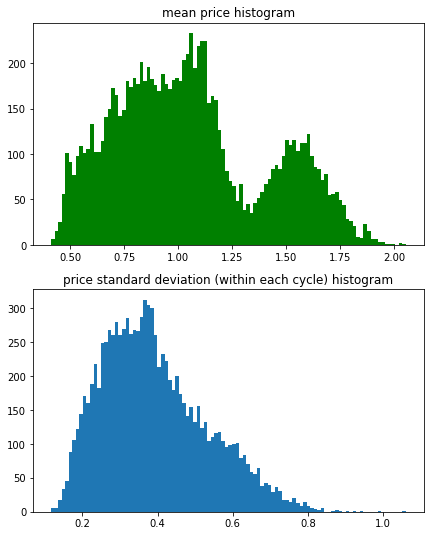
\includegraphics[width=0.6\textwidth]{output_3_2.png}}
\caption{Simplified Hayekian case: (i) an example of final demand and offer curves, (ii) the history of mean prices tick-by-tick, (iii) their coefficients of variation within each tick (cycle)}
\label{output_3_2.png}
\end{center}
\end{figure}

The \emph{coefficient of variation} at time $t$ is calculated as: $$\frac{standard~deviation_t}{mean_t}$$.

\begin{figure}[H]
\begin{center}
\fbox{\centering 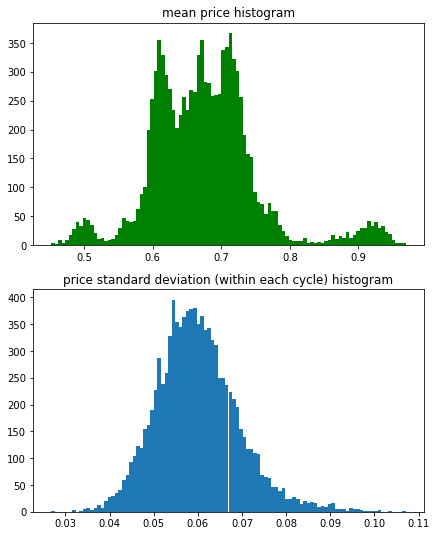
\includegraphics[width=0.6\textwidth]{output_3_3.png}}
\caption{Simplified Hayekian case: (i) the distribution of mean prices of each cycle (i.e., tick-by-tick) and (ii) that of their standard deviations within each tick (cycle)}
\label{output_3_3.png}
\end{center}
\end{figure}

\begin{center}
\fbox{\parbox[c][3.5cm][c]{11cm}{
A comment: we have a plausible series of mean prices, with a complicated behavior, and with a high stability of the dispersion of the values within each cycle.

The right side of the buyer and seller curves shows another plausible situation: that of the presence of agents not exchanging. {\color{red}A note for Matteo and Pietro: this is a very important emergent effect for the \href{https://terna.github.io/oligopoly/}{\emph{Oligopoly}} model.}}}
\end{center}

\bigskip

Have a look to the Appendix \ref{Two cases of not balancing numbers of buyers and sellers} for the cases of not balancing number of buyers and sellers.

The IPython (or Python 3.x) code is:

\begin{lstlisting}[language=Python, caption=The model in the simplified hayekian perspective, basicstyle=\ttfamily\footnotesize]
# hayekian perspective

warmingUp()

out = Output()
display(out)

meanPrice_ts=[]
meanPriceStDev_ts=[]
meanPriceVar_ts=[]

if usingRatios and not usingSqueezeRate:
    if buyersSellersRatio>1: d2*=sellersBuyersRatio
    if sellersBuyersRatio>1: d1*=buyersSellersRatio
        
if usingRatios and usingSqueezeRate:
    if buyersSellersRatio>1: d2*=sellersBuyersRatio*squeezeRate
    if sellersBuyersRatio>1: d1*=buyersSellersRatio*squeezeRate
    

for t in range(1,nCycles+1):    
    dealPrices=[]
    agNum=max(nBuyers,nSellers)

    for n in range(agNum):

        i = np.random.randint(0,nBuyers)
        j = np.random.randint(0,nSellers)
        
        if buyerPriceList[i]>=sellerPriceList[j]:
            dealPrices.append(sellerPriceList[j])
            buyerPriceList[i] *=1/(1+np.random.uniform(0,d1))
            sellerPriceList[j]*=1+np.random.uniform(0,d2)
        else:
            buyerPriceList[i] *=1+np.random.uniform(0,d1)
            sellerPriceList[j]*=1/(1+np.random.uniform(0,d2))
           
    if len(dealPrices) > 2:
        meanPrice_ts.append(s.mean(dealPrices))
        meanPriceVar_ts.append(s.variance(dealPrices))
        meanPriceStDev_ts.append(s.stdev(dealPrices))
    else:
        meanPrice_ts.append(np.nan)
        meanPriceStDev_ts.append(np.nan)

    if t % 1000==0:
        with out:
            clear_output()
        with out:
            print('time', t, 'and n. of exchanges in the last cycle', \
              len(dealPrices))
            print(\
        'mean and var of exchange prices in the last cycle: %1.3e, %1.3e' %\
              (meanPrice_ts[-1],meanPriceVar_ts[-1]))

        plt.figure(1,figsize=(7,15),clear=True)

        plt.subplot(311)
        plt.plot(sorted(buyerPriceList,reverse=True),"r")
        plt.plot(sorted(sellerPriceList),"b")
        plt.title(\
            "buyers' prices (red) and sellers' prices (blue)")
        xlabel("the agents")
        ylabel("agents' reservation prices")

        plt.subplot(312)
        plt.title("mean price of each cycle")
        xlabel("t")
        ylabel("mean price of each cycle")
        plt.plot(meanPrice_ts,"g")
        
        plt.subplot(313)
        plt.title("price coef. of variation within each cycle")
        coefOfVariation=[]
        for m in range(len(meanPriceStDev_ts)):
            coefOfVariation.append(meanPriceStDev_ts[m]/
                                   meanPrice_ts[m])
        plt.plot(coefOfVariation,".",markersize=0.1)
        xlabel("t")
        ylabel("price coef. of variation within each cycle")
        #time.sleep(0.1)

# hist crashes with NaN
meanPrice_ts_hist=[]
for k in range(len(meanPrice_ts)): 
    if not math.isnan(meanPrice_ts[k]):
        meanPrice_ts_hist.append(meanPrice_ts[k])
meanPriceStDev_ts_hist=[]
for k in range(len(meanPriceStDev_ts)): 
    if not math.isnan(meanPriceStDev_ts[k]):
        meanPriceStDev_ts_hist.append(meanPriceStDev_ts[k])
plt.figure(2,figsize=(7,9))
plt.subplot(211)
if meanPrice_ts_hist != []:
    plt.title("mean price histogram")
    plt.hist(meanPrice_ts_hist,100,color="g");
plt.subplot(212)
if meanPriceStDev_ts_hist != []:
    plt.title("price standard deviation (within each cycle) histogram")
    plt.hist(meanPriceStDev_ts_hist,100);
\end{lstlisting}


%%%%%%%%%%%%%%%%%%%%%%%%%%%%%%%%%%%%%%%%%%%%
\section{The unstructured version}\label{The unstructured version}\index{unstructured version}

The buyers and the sellers meet randomly as in Section \ref{The hayekian version}. Buyer $i$ and seller $j$ exchange in any case; the deal is recorded at the mean of the price of the seller $pL^s_j$ and of the price $pL^b_i$ of the buyer.

In this version the running prices are  are multiplied in each cycle by the following  correction coefficients:

\begin{itemize}

\item with the same probability for the buyer: (i) $c_b=\frac{1} {1 + u_b}$ or (ii) $c_b=1 + u_b$); in (i) and (ii) we have $u_b\sim\mathcal{U}(0,d_1)$

\item  with the same probability for the seller: (iii) $c_s=1 + u_s$ or (iv) $c_s=\frac{1} {1 + u_s}$; in (iii) and (iv) we have $u_s\sim\mathcal{U}(0,d_2)$.
\end{itemize}

With $seed=111$, $d_1=0.2$, $d_2=0.2$ and $nCycles$ set to $10,000$ we obtain exploding sequences of the means of the prices (mean in each cycle), and exploding standard deviation within each cycle (see Fig. \ref{output_4_2.png} and \ref{output_4_3.png}).

\begin{figure}[H]
\begin{center}
\fbox{\centering 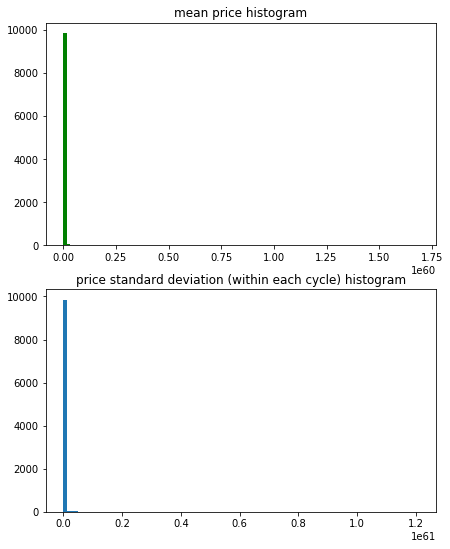
\includegraphics[width=0.6\textwidth]{output_4_2.png}}
\caption{Unstructured case: ((i) an example of final demand and offer curves, (ii) the history of mean prices tick-by-tick, (iii) their coefficients of variation within each tick (cycle)}
\label{output_4_2.png}
\end{center}
\end{figure}

The \emph{coefficient of variation} at time $t$ is calculated as: $$\frac{standard~deviation_t}{mean_t}$$.

\begin{figure}[H]
\begin{center}
\fbox{\centering 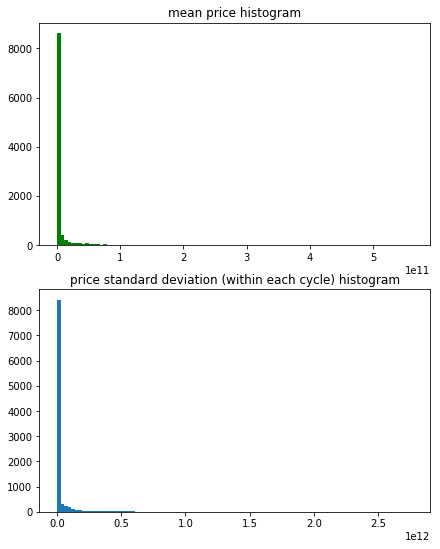
\includegraphics[width=0.6\textwidth]{output_4_3.png}}
\caption{Unstructured case: (i) the distribution of mean prices of each cycle (i.e., tick-by-tick) and (ii) that of their standard deviations within each tick (cycle)}
\label{output_4_3.png}
\end{center}
\end{figure}

\begin{center}
\fbox{\parbox[c][2.6cm][c]{10cm}{
A comment: this counter-example shows that, missing the \emph{intelligence} in the correction of the prices (implicitly propagating among all the agents), a system of pure random price settings is absolutely far from being plausible.}}
\end{center}

\bigskip

The IPython (or Python 3.x) code is:

\begin{lstlisting}[language=Python, caption=The unstructured version, basicstyle=\ttfamily\footnotesize]
# unstructured case

warmingUp()

out = Output()
display(out)

meanPrice_ts=[]
meanPriceStDev_ts=[]
meanPriceVar_ts=[]

if usingRatios and not usingSqueezeRate:
    if buyersSellersRatio>1: d2*=sellersBuyersRatio
    if sellersBuyersRatio>1: d1*=buyersSellersRatio
        
if usingRatios and usingSqueezeRate:
    if buyersSellersRatio>1: d2*=sellersBuyersRatio*squeezeRate
    if sellersBuyersRatio>1: d1*=buyersSellersRatio*squeezeRate

for t in range(1,nCycles+1):    
    dealPrices=[]
    agNum=max(nBuyers,nSellers)
    for n in range(agNum):
        i = np.random.randint(0,nBuyers)
        j = np.random.randint(0,nSellers)

        dealPrices.append((sellerPriceList[j]+buyerPriceList[i]/0.5))

        if np.random.uniform(0,1)>=0.5:    
            buyerPriceList[i] *=1/(1+np.random.uniform(0,d1))
            sellerPriceList[j]*=1+np.random.uniform(0,d2)
        else:
            buyerPriceList[i] *=1+np.random.uniform(0,d1)
            sellerPriceList[j]*=1/(1+np.random.uniform(0,d2))
        
           
    if len(dealPrices) > 2:
        meanPrice_ts.append(s.mean(dealPrices))
        meanPriceVar_ts.append(s.variance(dealPrices))
        meanPriceStDev_ts.append(s.stdev(dealPrices))
    else:
        meanPrice_ts.append(np.nan)
        meanPriceStDev_ts.append(np.nan)

    if t % 1000==0:
        with out:
            clear_output()
        with out:
            print('time', t, 'and n. of exchanges in the last cycle', \
              len(dealPrices))
            print(\
        'mean and var of exchange prices in the last cycle: %1.3e, %1.3e' %\
              (meanPrice_ts[-1],meanPriceVar_ts[-1]))

        plt.figure(3,figsize=(7,15),clear=True)

        plt.subplot(311)
        plt.plot(sorted(buyerPriceList,reverse=True),"r")
        plt.plot(sorted(sellerPriceList),"b")
        plt.title(\
            "buyers' prices (red) and sellers' prices (blue)")
        xlabel("the agents")
        ylabel("agents' reservation prices")

        plt.subplot(312)
        plt.title("mean price of each cycle")
        xlabel("t")
        ylabel("mean price of each cycle")
        plt.plot(meanPrice_ts,"g")
        
        plt.subplot(313)
        plt.title("price coef. of variation within each cycle")
        coefOfVariation=[]
        for m in range(len(meanPriceStDev_ts)):
            coefOfVariation.append(meanPriceStDev_ts[m]/
                                   meanPrice_ts[m])
        plt.plot(coefOfVariation,".",markersize=0.1)
        xlabel("t")
        ylabel("price coef. of variation within each cycle")
        #time.sleep(0.1)

# hist crashes with NaN
meanPrice_ts_hist=[]
for k in range(len(meanPrice_ts)): 
    if not math.isnan(meanPrice_ts[k]):
        meanPrice_ts_hist.append(meanPrice_ts[k])
meanPriceStDev_ts_hist=[]
for k in range(len(meanPriceStDev_ts)): 
    if not math.isnan(meanPriceStDev_ts[k]):
        meanPriceStDev_ts_hist.append(meanPriceStDev_ts[k])
plt.figure(4,figsize=(7,9))
plt.subplot(211)
if meanPrice_ts_hist != []:
    plt.title("mean price histogram")
    plt.hist(meanPrice_ts_hist,100,color="g");
plt.subplot(212)
if meanPriceStDev_ts_hist != []:
    plt.title("price standard deviation (within each cycle) histogram")
    plt.hist(meanPriceStDev_ts_hist,100);
\end{lstlisting}




\renewcommand{\thesubsection}{\thesection.\alph{subsection}}
\renewcommand{\thesection}{\thechapter.\arabic{section}}

\begin{appendices}

%%%%%%%%%%%%%%%%%%%%%%%%%%%%%%%%%%%%%%%%%%%%
%%%%%%%%%%%%%%%%%%%%%%%%%%%%%%%%%%%%%%%%%%%%
\chapter{Two triple cases of not balancing numbers of buyers and sellers}\index{not balancing number of buyers and sellers}\label{Two triple cases of not balancing numbers of buyers and sellers}
\thispagestyle{fancy}

%%%%%%%%%%%%%%%%%%%%%%%%%%%%%%%%%%%%%%%%%%%%
\section{Case $nBuyers \gg nSellers$}
With $nBuyers \gg nSellers$ (e.g., $nBuyers=100$ and $nSellers=50$, as in Fig. \ref{output_3_1a.png}), we have three possible paths of analysis. 

%%%%%%%%%%%%%%%%%%%%%%%%%%%%%%%%%%%%%%%%%%%%
\subsection{Case $nBuyers \gg nSellers$, with different rates of per-capita correction}\label{nBuyers > nSellers with different rates of per-capita correction}\index{nBuyers > nSellers with different rates of per-capita correction}

If $nBuyers \gg nSellers$, we have in each cycle one call---in mean---to a  \emph{seller} from each  \emph{buyer}, the number of per-capita actions of the \emph{sellers} in each cycle is greater of the number of per-capita actions of the \emph{buyers}.

As a consequence, the probability that a \emph{seller} decreases her price to meet that of a \emph{b}uyer is greater than the probability that a \emph{buyer} increases her price to meet that of a \emph{seller}. 

We can observe that in Figs. \ref{output_3_2a.png} and \ref{output_3_3a.png} the prices are---in the end---lower than in Figs. \ref{output_3_2.png} and \ref{output_3_3.png} and, must of all, the price tendency has a strong negative slope. We always have $d_0=0.1$, $d_1=0.2$,  $d_2=0.2$, and $seed=111$.

This result is inconsistent with the microeconomic theory, where we could expect that an excess of demand will generate the rise of the prices.

\begin{figure}[H]
\begin{center}
\fbox{\centering 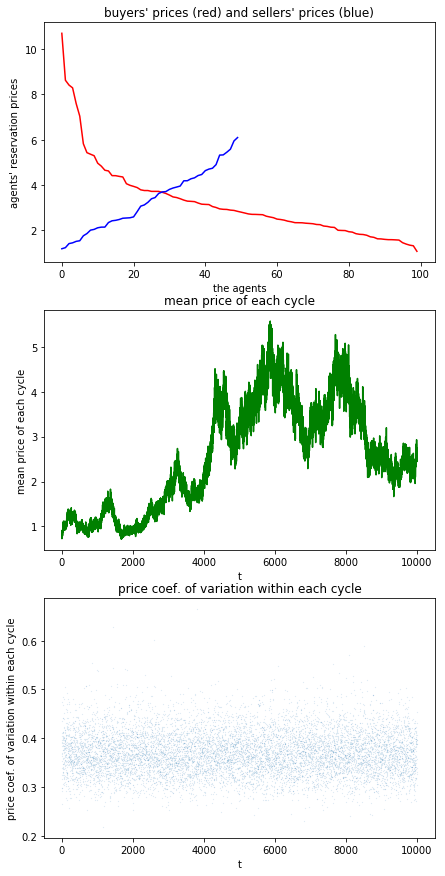
\includegraphics[width=0.4\textwidth]{output_3_1a.png}}
\caption{An example of initial not overlapping demand curve and offer curve, case $nBuyers \gg nSellers$}
\label{output_3_1a.png}
\end{center}
\end{figure}

\begin{figure}[H]
\begin{center}
\fbox{\centering 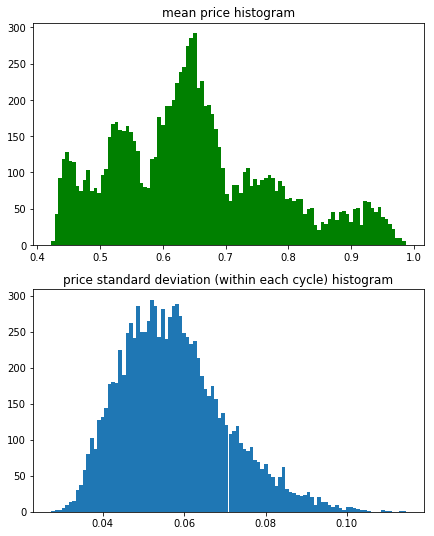
\includegraphics[width=0.4\textwidth]{output_3_2a.png}}
\caption{Simplified Hayekian case, with $nBuyers \gg nSellers$: (i) an example of final demand and offer curves, (ii) the history of mean prices tick-by-tick, (iii) their coefficients of variation within each tick (cycle)}
\label{output_3_2a.png}
\end{center}
\end{figure}

\begin{figure}[H]
\begin{center}
\fbox{\centering 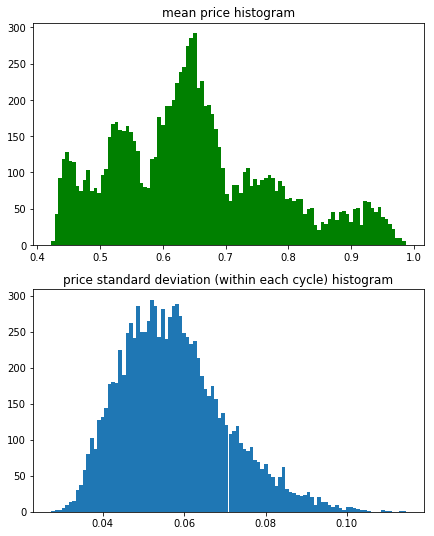
\includegraphics[width=0.4\textwidth]{output_3_3a.png}}
\caption{Simplified Hayekian case, with $nBuyers \gg nSellers$: (i) the distribution of mean prices of each cycle (i.e., tick-by-tick) and (ii) that of their standard deviations within each tick (cycle)}
\label{output_3_3a.png}
\end{center}
\end{figure}

%%%%%%%%%%%%%%%%%%%%%%%%%%%%%%%%%%%%%%%%%%%%
\subsection{Case $nBuyers \gg nSellers$, with unequal rates of per-capita correction, with equivalent effects}\label{nBuyers > nSellers with unequal rates of per-capita correction, with equivalent effects}\index{nBuyers > nSellers with unequal rates of per-capita correction, with equivalent effects}

Again, with $nBuyers \gg nSellers$, and always having in each cycle one call---in mean---to a  \emph{seller} from each  \emph{buyer}, the number of per-capita actions of the \emph{sellers} in each cycle is greater of the number of per-capita actions of the \emph{buyers}.

In this second version of the case $nBuyers \gg nSellers$, we always have $d_0=0.1$, $d_1=0.2$,  $d_2=0.2$, and $seed=111$.

The novelty is that of setting $usingRatios=True$, so we are activating limitations to $d_1$ or $d_2$.

The limitations work as follow:
\begin{itemize}

\item if the $\frac{nBuyers}{nSellers}>1$ (our case in this example), $d_2$, i.e. the upper limit of the rate of correction of the price of the sellers, is multiplied by $\frac{nSellers}{nBuyers}$;\footnote{An example to clarify: in this Section we have $nBuyers=100$ and $nSellers=50$, so $\frac{nBuyers}{nSellers} \equiv 2$ and $\frac{nSellers}{nBuyers} \equiv 0.5$; $d_2$ is reduced of the 50\%.}

\item if the $\frac{nSellers}{nBuyers}>1$, $d_1$, i.e. the upper limit of the rate of correction of the price of the buyers, is multiplied by $\frac{nBuyers}{nSellers}$.

\end{itemize}

We have now unequal rates of per-capita correction, with equivalent effects. The interpretation is that if the number of sellers is smaller than the number of buyers, the sellers act with a slow pace of price correction (proportional to $\frac{nSellers}{nBuyers}$) because in this way they can cherry-pick the best buyers (those with the higher reservation price). In this way, they avoid to contribute to the fall of the prices.

Always with Fig. \ref{output_3_1a.png} as the starting configuration of the prices, in Fig.s \ref{output_3_2aa.png} and \ref{output_3_3aa.png} we see now interesting price oscillations roughly confined between the limits of Fig. \ref{output_3_1a.png}. 


\begin{figure}[H]
\begin{center}
\fbox{\centering 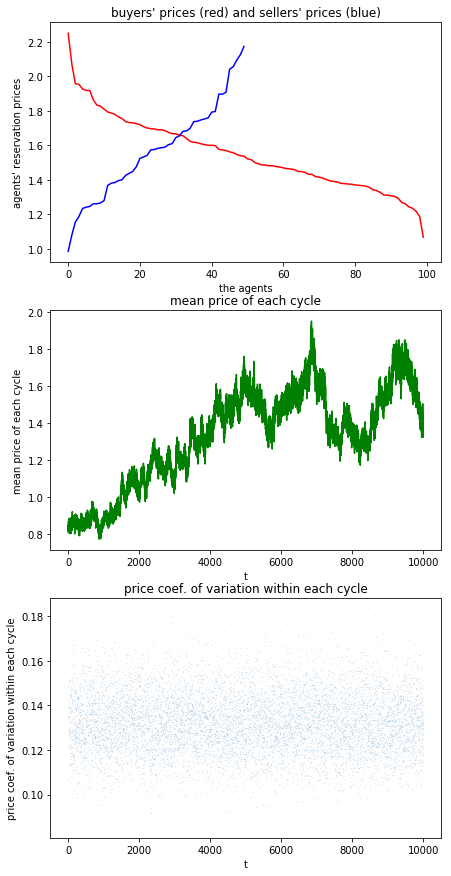
\includegraphics[width=0.4\textwidth]{output_3_2aa.png}}
\caption{Simplified Hayekian case, with $nBuyers \gg nSellers$ but with equivalent effects: (i) an example of final demand and offer curves, (ii) the history of mean prices tick-by-tick, (iii) their coefficients of variation within each tick (cycle)}
\label{output_3_2aa.png}
\end{center}
\end{figure}

\begin{figure}[H]
\begin{center}
\fbox{\centering 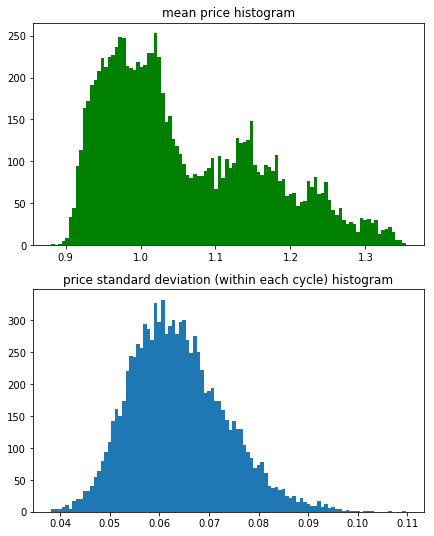
\includegraphics[width=0.4\textwidth]{output_3_3aa.png}}
\caption{Simplified Hayekian case, with $nBuyers \gg nSellers$ but with equivalent effects: (i) the distribution of mean prices of each cycle (i.e., tick-by-tick) and (ii) that of their standard deviations within each tick (cycle)}
\label{output_3_3aa.png}
\end{center}
\end{figure}

%%%%%%%%%%%%%%%%%%%%%%%%%%%%%%%%%%%%%%%%%%%%
\subsection{Case $nBuyers \gg nSellers$, with unequal rates of per-capita correction, but squeezing the effects}\label{nBuyers > nSellers with unequal rates of per-capita correction, but squeezing the effects}\index{nBuyers > nSellers with unequal rates of per-capita correction, but squeezing the effects}

In this third version of the case $nBuyers \gg nSellers$, we always have $d_0=0.1$, $d_1=0.2$,  $d_2=0.2$, and $seed=111$.

The second novelty, after that of Section \ref{nBuyers > nSellers with unequal rates of per-capita correction, with equivalent effects}, is that of setting $usingSqueeze=True$ (and setting $usingRatios=True$ as in Section  \ref{nBuyers > nSellers with unequal rates of per-capita correction, with equivalent effects}), so we are activating further limitations to $d_1$ or $d_2$. We also have $squeezeRate=0.3$.

\begin{itemize}

\item if the $\frac{nBuyers}{nSellers}>1$ (our case in this example), $d_2$, i.e. the upper limit of the rate of correction of the price of the sellers, is multiplied by $squeezeRate$;

\item if the $\frac{nSellers}{nBuyers}>1$, $d_1$, i.e. the upper limit of the rate of correction of the price of the buyers, is multiplied by $squeezeRate$;
\end{itemize}


Always with Fig. \ref{output_3_1a.png} as the starting configuration of the prices, in Fig.s \ref{output_3_2aaa.png} and \ref{output_3_3aaa.png} we see a limited price dynamics, very close to the top band of Fig. \ref{output_3_1a.png}. This result is perfectly consistent with microeconomic theory.

\begin{figure}[H]
\begin{center}
\fbox{\centering 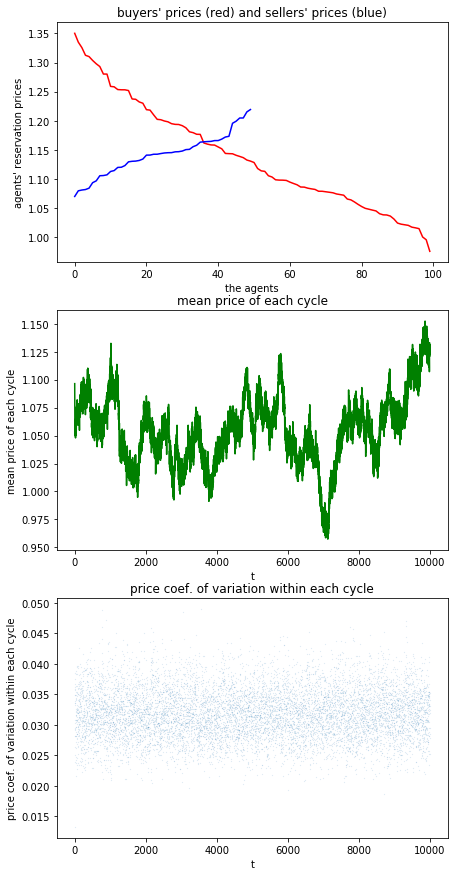
\includegraphics[width=0.4\textwidth]{output_3_2aaa.png}}
\caption{Simplified Hayekian case, with $nBuyers \gg nSellers$ but squeezing the effects: (i) an example of final demand and offer curves, (ii) the history of mean prices tick-by-tick, (iii) their coefficients of variation within each tick (cycle)}
\label{output_3_2aaa.png}
\end{center}
\end{figure}

\begin{figure}[H]
\begin{center}
\fbox{\centering 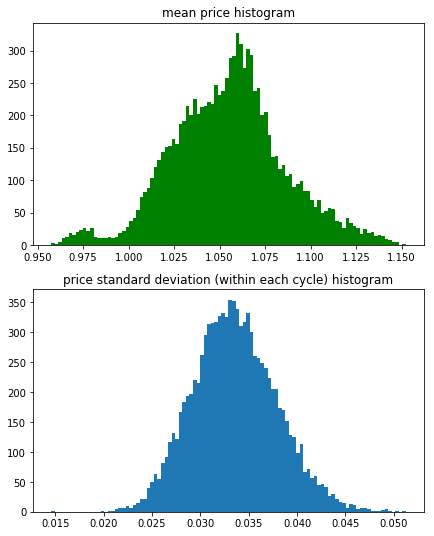
\includegraphics[width=0.4\textwidth]{output_3_3aaa.png}}
\caption{Simplified Hayekian case, with $nBuyers \gg nSellers$ but squeezing the effects: (i) the distribution of mean prices of each cycle (i.e., tick-by-tick) and (ii) that of their standard deviations within each tick (cycle)}
\label{output_3_3aaa.png}
\end{center}
\end{figure}


%%%%%%%%%%%%%%%%%%%%%%%%%%%%%%%%%%%%%%%%%%%%
\section{Case $nBuyers \ll nSellers$}
With $nBuyers \ll nSellers$ (e.g., $nBuyers=50$ and $nSellers=100$, as in Fig. \ref{output_3_1b.png}), we again have three possible paths of analysis. 

%%%%%%%%%%%%%%%%%%%%%%%%%%%%%%%%%%%%%%%%%%%%
\subsection{Case $nBuyers \ll nSellers$, with different rates of per-capita correction}\label{nBuyers < nSellers with different rates of per-capita correction}\index{nBuyers < nSellers with different rates of per-capita correction}

If $nBuyers \ll nSellers$, we have in each cycle one call---in mean---to a  \emph{buyer} from each  \emph{seller}, the number of per-capita actions of the \emph{buyers} in each cycle is greater of the number of per-capita actions of the \emph{sellers}.

As a consequence, the probability that a \emph{buyer} increases her price to meet that of a \emph{seller} is greater than the probability that a \emph{seller} decreases her price to meet that of a \emph{buyer}. 

We can observe that in Figs. \ref{output_3_2b.png} and \ref{output_3_3b.png} the prices are---in the end---greater than in Figs. \ref{output_3_2.png} and \ref{output_3_3.png} and, must of all, the price tendence has a strong positive slope. We always have $d_0=0.1$, $d_1=0.2$,  $d_2=0.2$, and $seed=111$.

This result is inconsistent with the microeconomic theory, where we could expect that an excess of offer will generate the fall of the prices.


\begin{figure}[H]
\begin{center}
\fbox{\centering 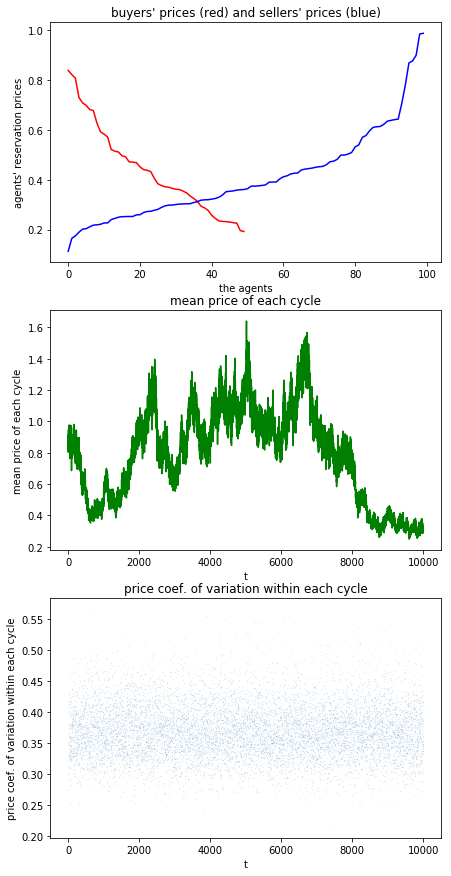
\includegraphics[width=0.4\textwidth]{output_3_1b.png}}
\caption{An example of initial not overlapping demand curve and offer curve, case $nBuyers \ll nSellers$}
\label{output_3_1b.png}
\end{center}
\end{figure}

\begin{figure}[H]
\begin{center}
\fbox{\centering 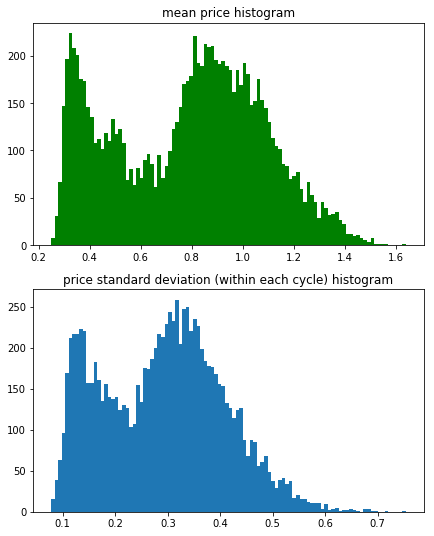
\includegraphics[width=0.4\textwidth]{output_3_2b.png}}
\caption{Simplified Hayekian case, with $nBuyers \ll nSellers$: (i) an example of final demand and offer curves, (ii) the history of mean prices tick-by-tick, (iii) their coefficients of variation within each tick (cycle)}
\label{output_3_2b.png}
\end{center}
\end{figure}

\begin{figure}[H]
\begin{center}
\fbox{\centering 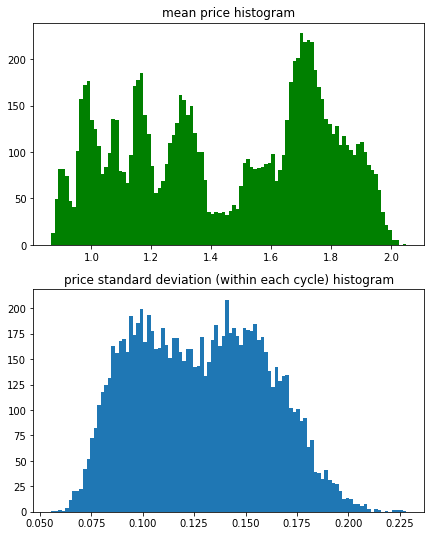
\includegraphics[width=0.4\textwidth]{output_3_3b.png}}
\caption{Simplified Hayekian case, with $nBuyers \ll nSellers$: (i) the distribution of mean prices of each cycle (i.e., tick-by-tick) and (ii) that of their standard deviations within each tick (cycle)}
\label{output_3_3b.png}
\end{center}
\end{figure}



%%%%%%%%%%%%%%%%%%%%%%%%%%%%%%%%%%%%%%%%%%%%
\subsection{Case $nBuyers \ll nSellers$, with unequal rates of per-capita correction, with equivalent effects}\label{nBuyers < nSellers with unequal rates of per-capita correction, with equivalent effects}\index{nBuyers < nSellers with unequal rates of per-capita correction, with equivalent effects}

In this second version of the case $nBuyers \ll nSellers$, we always have $d_0=0.1$, $d_1=0.2$,  $d_2=0.2$, and $seed=111$.

As in Section \ref{nBuyers > nSellers with unequal rates of per-capita correction, with equivalent effects}, the novelty is that of setting $usingRatios=True$, so we are activating limitations to $d_1$ or $d_2$.

The limitations work as follow:
\begin{itemize}

\item if the $\frac{nBuyers}{nSellers}>1$, $d_2$, i.e. the upper limit of the rate of correction of the price of the sellers, is multiplied by $\frac{nSellers}{nBuyers}$;

\item if the $\frac{nSellers}{nBuyers}>1$ (our case in this example), $d_1$, i.e. the upper limit of the rate of correction of the price of the buyers, is multiplied by $\frac{nBuyers}{nSellers}$.\footnote{An example to clarify: in this Section we have $nBuyers=50$ and $nSellers=100$, so $\frac{nSellers}{nBuyers} \equiv 2$ and $\frac{nBuyers}{nSellers} \equiv0.5$; $d_1$ is reduced of the 50\%.}

\end{itemize}

We have now unequal rates of per-capita correction, with equivalent effects. The interpretation is that if the number of buyers is smaller than the number of sellers, the buyers act with a slow pace of price correction (proportional to $\frac{nBuyers}{nSellers}$) because in this way they can cherry-pick the best sellers (those with the lower reservation price). In this way, they avoid to contribute to the rise of the prices.

Always with Fig. \ref{output_3_1b.png} as the starting configuration of the prices, in Fig.s \ref{output_3_2bb.png} and \ref{output_3_3bb.png} we see now a compressed price oscillations roughly close to the bottom limits of Fig. \ref{output_3_1b.png}.

\begin{figure}[H]
\begin{center}
\fbox{\centering 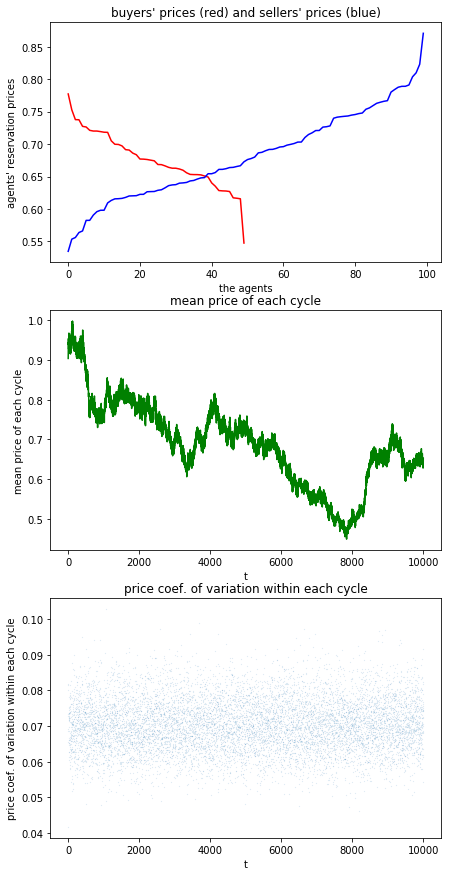
\includegraphics[width=0.4\textwidth]{output_3_2bb.png}}
\caption{Simplified Hayekian case, with $nBuyers \gg nSellers$ with equivalent effects: (i) an example of final demand and offer curves, (ii) the history of mean prices tick-by-tick, (iii) their coefficients of variation within each tick (cycle)}
\label{output_3_2bb.png}
\end{center}
\end{figure}

\begin{figure}[H]
\begin{center}
\fbox{\centering 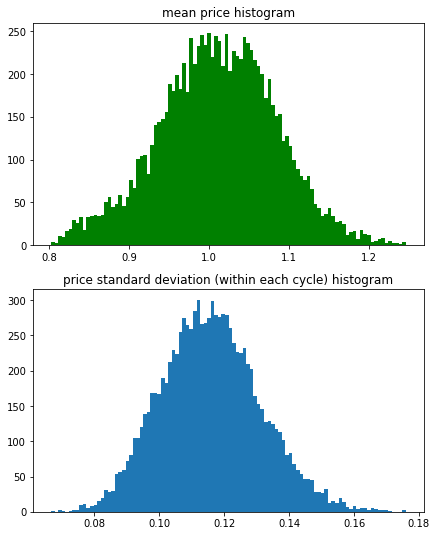
\includegraphics[width=0.4\textwidth]{output_3_3bb.png}}
\caption{Simplified Hayekian case, with $nBuyers \gg nSellers$ but with equivalent effects: (i) the distribution of mean prices of each cycle (i.e., tick-by-tick) and (ii) that of their standard deviations within each tick (cycle)}
\label{output_3_3bb.png}
\end{center}
\end{figure}


%%%%%%%%%%%%%%%%%%%%%%%%%%%%%%%%%%%%%%%%%%%%
\subsection{Case $nBuyers \ll nSellers$, with unequal rates of per-capita correction, but squeezing the effects}\label{nBuyers < nSellerswith unequal rates of per-capita correction, but squeezing the effects}\index{nBuyers < nSellers with unequal rates of per-capita correction, but squeezing the effects}

In this third version of the case $nBuyers \ll nSellers$, we always have $d_0=0.1$, $d_1=0.2$,  $d_2=0.2$, and $seed=111$.

The second novelty, after that of Section \ref{nBuyers < nSellers with unequal rates of per-capita correction, with equivalent effects}, is that of setting $usingSqueeze=True$ (and setting $usingRatios=True$ as in Section  \ref{nBuyers < nSellers with unequal rates of per-capita correction, with equivalent effects}), so we are activating further limitations to $d_1$ or $d_2$. We also have $squeezeRate=0.3$.

\begin{itemize}

\item if the $\frac{nBuyers}{nSellers}>1$, $d_2$, i.e. the upper limit of the rate of correction of the price of the sellers, is multiplied by $squeezeRate$;

\item if the $\frac{nSellers}{nBuyers}>1$ (our case in this example), $d_1$, i.e. the upper limit of the rate of correction of the price of the buyers, is multiplied by $squeezeRate$;
\end{itemize}


Always with Fig. \ref{output_3_1b.png} as the starting configuration of the prices, in Fig.s \ref{output_3_2bbb.png} and \ref{output_3_3bbb.png} we see a limited price dynamics, very close to the bottom band of Fig. \ref{output_3_1b.png}. This result is perfectly consistent with microeconomic theory.

\begin{figure}[H]
\begin{center}
\fbox{\centering 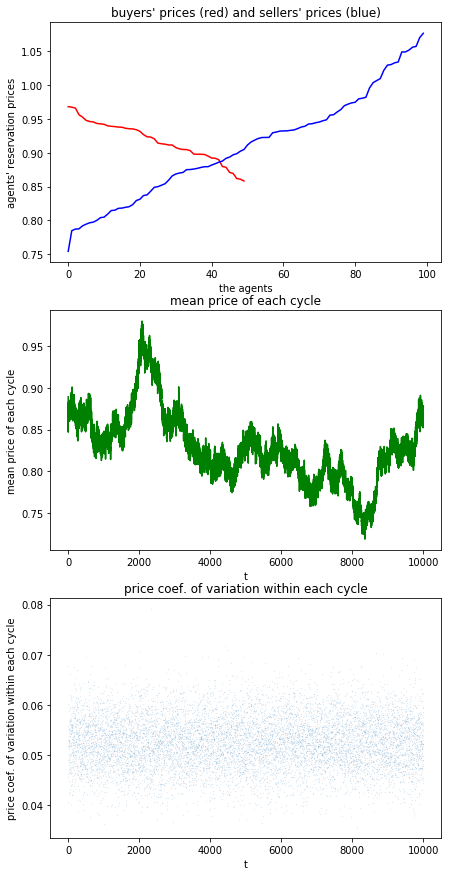
\includegraphics[width=0.4\textwidth]{output_3_2bbb.png}}
\caption{Simplified Hayekian case, with $nBuyers \gg nSellers$ but squeezing the effects: (i) an example of final demand and offer curves, (ii) the history of mean prices tick-by-tick, (iii) their coefficients of variation within each tick (cycle)}
\label{output_3_2bbb.png}
\end{center}
\end{figure}

\begin{figure}[H]
\begin{center}
\fbox{\centering 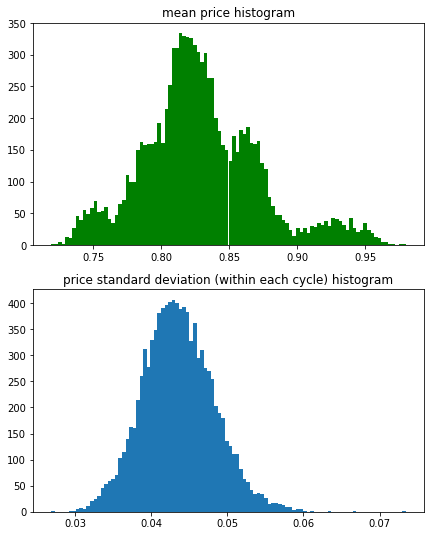
\includegraphics[width=0.4\textwidth]{output_3_3bbb.png}}
\caption{Simplified Hayekian case, with $nBuyers \gg nSellers$ but squeezing the effects: (i) the distribution of mean prices of each cycle (i.e., tick-by-tick) and (ii) that of their standard deviations within each tick (cycle)}
\label{output_3_3bbb.png}
\end{center}
\end{figure}


%%%%%%%%%%%%%%%%%%%%%%%%%%%%%%%%%%%%%%%%%%%%
%%%%%%%%%%%%%%%%%%%%%%%%%%%%%%%%%%%%%%%%%%%%
\chapter{Activating \emph{idle} agents}\index{idle agents}\label{Activating idle agents}
\thispagestyle{fancy}



\end{appendices}

\clearpage
\addcontentsline{toc}{chapter}{Bibliography}
\bibliography{./bibliografiaGenerale}
\bibliographystyle{plainnatmm}


\clearpage
\addcontentsline{toc}{chapter}{Index}
\printindex


\end{document}  





